% Options for packages loaded elsewhere
\PassOptionsToPackage{unicode}{hyperref}
\PassOptionsToPackage{hyphens}{url}
%
\documentclass[
  ignorenonframetext,
]{beamer}
\usepackage{pgfpages}
\setbeamertemplate{caption}[numbered]
\setbeamertemplate{caption label separator}{: }
\setbeamercolor{caption name}{fg=normal text.fg}
\beamertemplatenavigationsymbolsempty
% Prevent slide breaks in the middle of a paragraph
\widowpenalties 1 10000
\raggedbottom
\setbeamertemplate{part page}{
  \centering
  \begin{beamercolorbox}[sep=16pt,center]{part title}
    \usebeamerfont{part title}\insertpart\par
  \end{beamercolorbox}
}
\setbeamertemplate{section page}{
  \centering
  \begin{beamercolorbox}[sep=12pt,center]{section title}
    \usebeamerfont{section title}\insertsection\par
  \end{beamercolorbox}
}
\setbeamertemplate{subsection page}{
  \centering
  \begin{beamercolorbox}[sep=8pt,center]{subsection title}
    \usebeamerfont{subsection title}\insertsubsection\par
  \end{beamercolorbox}
}
\AtBeginPart{
  \frame{\partpage}
}
\AtBeginSection{
  \ifbibliography
  \else
    \frame{\sectionpage}
  \fi
}
\AtBeginSubsection{
  \frame{\subsectionpage}
}

\usepackage{amsmath,amssymb}
\usepackage{iftex}
\ifPDFTeX
  \usepackage[T1]{fontenc}
  \usepackage[utf8]{inputenc}
  \usepackage{textcomp} % provide euro and other symbols
\else % if luatex or xetex
  \usepackage{unicode-math}
  \defaultfontfeatures{Scale=MatchLowercase}
  \defaultfontfeatures[\rmfamily]{Ligatures=TeX,Scale=1}
\fi
\usepackage{lmodern}
\ifPDFTeX\else  
    % xetex/luatex font selection
\fi
% Use upquote if available, for straight quotes in verbatim environments
\IfFileExists{upquote.sty}{\usepackage{upquote}}{}
\IfFileExists{microtype.sty}{% use microtype if available
  \usepackage[]{microtype}
  \UseMicrotypeSet[protrusion]{basicmath} % disable protrusion for tt fonts
}{}
\makeatletter
\@ifundefined{KOMAClassName}{% if non-KOMA class
  \IfFileExists{parskip.sty}{%
    \usepackage{parskip}
  }{% else
    \setlength{\parindent}{0pt}
    \setlength{\parskip}{6pt plus 2pt minus 1pt}}
}{% if KOMA class
  \KOMAoptions{parskip=half}}
\makeatother
\usepackage{xcolor}
\newif\ifbibliography
\setlength{\emergencystretch}{3em} % prevent overfull lines
\setcounter{secnumdepth}{-\maxdimen} % remove section numbering


\providecommand{\tightlist}{%
  \setlength{\itemsep}{0pt}\setlength{\parskip}{0pt}}\usepackage{longtable,booktabs,array}
\usepackage{calc} % for calculating minipage widths
\usepackage{caption}
% Make caption package work with longtable
\makeatletter
\def\fnum@table{\tablename~\thetable}
\makeatother
\usepackage{graphicx}
\makeatletter
\newsavebox\pandoc@box
\newcommand*\pandocbounded[1]{% scales image to fit in text height/width
  \sbox\pandoc@box{#1}%
  \Gscale@div\@tempa{\textheight}{\dimexpr\ht\pandoc@box+\dp\pandoc@box\relax}%
  \Gscale@div\@tempb{\linewidth}{\wd\pandoc@box}%
  \ifdim\@tempb\p@<\@tempa\p@\let\@tempa\@tempb\fi% select the smaller of both
  \ifdim\@tempa\p@<\p@\scalebox{\@tempa}{\usebox\pandoc@box}%
  \else\usebox{\pandoc@box}%
  \fi%
}
% Set default figure placement to htbp
\def\fps@figure{htbp}
\makeatother
% definitions for citeproc citations
\NewDocumentCommand\citeproctext{}{}
\NewDocumentCommand\citeproc{mm}{%
  \begingroup\def\citeproctext{#2}\cite{#1}\endgroup}
\makeatletter
 % allow citations to break across lines
 \let\@cite@ofmt\@firstofone
 % avoid brackets around text for \cite:
 \def\@biblabel#1{}
 \def\@cite#1#2{{#1\if@tempswa , #2\fi}}
\makeatother
\newlength{\cslhangindent}
\setlength{\cslhangindent}{1.5em}
\newlength{\csllabelwidth}
\setlength{\csllabelwidth}{3em}
\newenvironment{CSLReferences}[2] % #1 hanging-indent, #2 entry-spacing
 {\begin{list}{}{%
  \setlength{\itemindent}{0pt}
  \setlength{\leftmargin}{0pt}
  \setlength{\parsep}{0pt}
  % turn on hanging indent if param 1 is 1
  \ifodd #1
   \setlength{\leftmargin}{\cslhangindent}
   \setlength{\itemindent}{-1\cslhangindent}
  \fi
  % set entry spacing
  \setlength{\itemsep}{#2\baselineskip}}}
 {\end{list}}
\usepackage{calc}
\newcommand{\CSLBlock}[1]{\hfill\break\parbox[t]{\linewidth}{\strut\ignorespaces#1\strut}}
\newcommand{\CSLLeftMargin}[1]{\parbox[t]{\csllabelwidth}{\strut#1\strut}}
\newcommand{\CSLRightInline}[1]{\parbox[t]{\linewidth - \csllabelwidth}{\strut#1\strut}}
\newcommand{\CSLIndent}[1]{\hspace{\cslhangindent}#1}

\usepackage{float}
\usepackage{tabularray}
\usepackage[normalem]{ulem}
\usepackage{graphicx}
\UseTblrLibrary{booktabs}
\UseTblrLibrary{rotating}
\UseTblrLibrary{siunitx}
\NewTableCommand{\tinytableDefineColor}[3]{\definecolor{#1}{#2}{#3}}
\newcommand{\tinytableTabularrayUnderline}[1]{\underline{#1}}
\newcommand{\tinytableTabularrayStrikeout}[1]{\sout{#1}}
\makeatletter
\@ifpackageloaded{caption}{}{\usepackage{caption}}
\AtBeginDocument{%
\ifdefined\contentsname
  \renewcommand*\contentsname{Table of contents}
\else
  \newcommand\contentsname{Table of contents}
\fi
\ifdefined\listfigurename
  \renewcommand*\listfigurename{List of Figures}
\else
  \newcommand\listfigurename{List of Figures}
\fi
\ifdefined\listtablename
  \renewcommand*\listtablename{List of Tables}
\else
  \newcommand\listtablename{List of Tables}
\fi
\ifdefined\figurename
  \renewcommand*\figurename{Figure}
\else
  \newcommand\figurename{Figure}
\fi
\ifdefined\tablename
  \renewcommand*\tablename{Table}
\else
  \newcommand\tablename{Table}
\fi
}
\@ifpackageloaded{float}{}{\usepackage{float}}
\floatstyle{ruled}
\@ifundefined{c@chapter}{\newfloat{codelisting}{h}{lop}}{\newfloat{codelisting}{h}{lop}[chapter]}
\floatname{codelisting}{Listing}
\newcommand*\listoflistings{\listof{codelisting}{List of Listings}}
\makeatother
\makeatletter
\makeatother
\makeatletter
\@ifpackageloaded{caption}{}{\usepackage{caption}}
\@ifpackageloaded{subcaption}{}{\usepackage{subcaption}}
\makeatother

\usepackage{bookmark}

\IfFileExists{xurl.sty}{\usepackage{xurl}}{} % add URL line breaks if available
\urlstyle{same} % disable monospaced font for URLs
\hypersetup{
  pdftitle={Tobacco excise in Indonesia},
  pdfauthor={Krisna Gupta},
  hidelinks,
  pdfcreator={LaTeX via pandoc}}


\title{Tobacco excise in Indonesia}
\author{Krisna Gupta}
\date{September 25, 2024}
\institute{Center for INdonesian Policy Studies}

\begin{document}
\frame{\titlepage}


\begin{frame}{Introduction}
\phantomsection\label{introduction}
\begin{itemize}
\item
  Nicotine is addictive and harmful. Controlling tobacco use via
  taxation requires understanding of demand elasticity of the good
  (Hidayat and Thabrany 2011).
\item
  Indonesian excise structure is complicated, with various bracket based
  on firms' production size and types of cigarettes.
\item
  It happes amid various target: demand control, revenue generation, and
  jobs generation.
\item
  In this project, we are tasked to see whether substitution happened.
\end{itemize}
\end{frame}

\begin{frame}{Tax structure}
\phantomsection\label{tax-structure}
\begin{longtable}[]{@{}
  >{\raggedright\arraybackslash}p{(\linewidth - 8\tabcolsep) * \real{0.2000}}
  >{\raggedright\arraybackslash}p{(\linewidth - 8\tabcolsep) * \real{0.2000}}
  >{\raggedright\arraybackslash}p{(\linewidth - 8\tabcolsep) * \real{0.2000}}
  >{\raggedright\arraybackslash}p{(\linewidth - 8\tabcolsep) * \real{0.2000}}
  >{\raggedright\arraybackslash}p{(\linewidth - 8\tabcolsep) * \real{0.2000}}@{}}
\toprule\noalign{}
\begin{minipage}[b]{\linewidth}\raggedright
type/category
\end{minipage} & \begin{minipage}[b]{\linewidth}\raggedright
Production
\end{minipage} & \begin{minipage}[b]{\linewidth}\raggedright
HJE (kIDR)
\end{minipage} & \begin{minipage}[b]{\linewidth}\raggedright
tariff (kIDR)
\end{minipage} & \begin{minipage}[b]{\linewidth}\raggedright
AVE(\%)
\end{minipage} \\
\midrule\noalign{}
\endhead
SKM1 & \textgreater{} 3 billion & 1.95 & .985 & 50.51 \\
SKM2 & \textless= 3 billion & 1.14 & .6 & 52.63 \\
SPM1 & \textgreater{} 3 billion & 2.005 & 1.065 & 53.12 \\
SPM2 & \textless= 3 billion & 1.135 & .635 & 55.94 \\
SKT1a & \textgreater{} 2 billion & \textgreater1.635 & .44 & 26.91 \\
SKT1b & \textgreater{} 2 billion & \textgreater1.135 & .345 & 30.4 \\
SKT2 & (0.5 \textless{} x \textless{} 2) billion & \textgreater600 &
.205 & 34.2 \\
SKT3 & \textless= 0.5 billion & \textgreater505 & .115 & 22.77 \\
\bottomrule\noalign{}
\end{longtable}
\end{frame}

\begin{frame}{The tax structure}
\phantomsection\label{the-tax-structure}
\begin{itemize}
\item
  The tax structure is lower than what WHO suggests (Prasetyo and
  Adrison 2020).
\item
  The ``job'' goal leads to a lower tax rate for lower production firm
  which encourage larger firms to shrink (or at least discourage small
  firms to go large)
\item
  The ``job creation'' goal may undermine the ``revenue'' goal and
  ``control'' goal.
\end{itemize}
\end{frame}

\begin{frame}{Data}
\phantomsection\label{data}
\begin{table}
\centering
\begin{tblr}[         %% tabularray outer open
]                     %% tabularray outer close
{                     %% tabularray inner open
colspec={Q[]Q[]Q[]Q[]Q[]},
column{1}={}{halign=l,},
column{2,3,4,5}={}{halign=r,},
}                     %% tabularray inner close
\toprule
& Mean & SD & N & Histogram \\ \midrule %% TinyTableHeader
qskm1 & 15272289807.50 & 5521195234.89 & 120 & ▄▆▆▆▇▆▆▂▁ \\
rskm1 & 9.5e+12 & 3.5e+12 & 120 & ▂▆▆▇▇▁▁▁ \\
tskm1 & 667.10 & 235.16 & 120 & ▅▂▇▂▂▂▂ \\
lskm1 & 1318.90 & 458.84 & 120 & ▅▂▇▅▂▂ \\
pskm1 & 1327.00 & 338.51 & 11 & ▇▃▃▇▃▇▃▃ \\
\bottomrule
\end{tblr}
\end{table}

We have monthly data on production and excise from 2014-2023 except for
market price. Small degree of freedom compared to the tax brackett.
\end{frame}

\begin{frame}{Market Prices}
\phantomsection\label{market-prices}
\pandocbounded{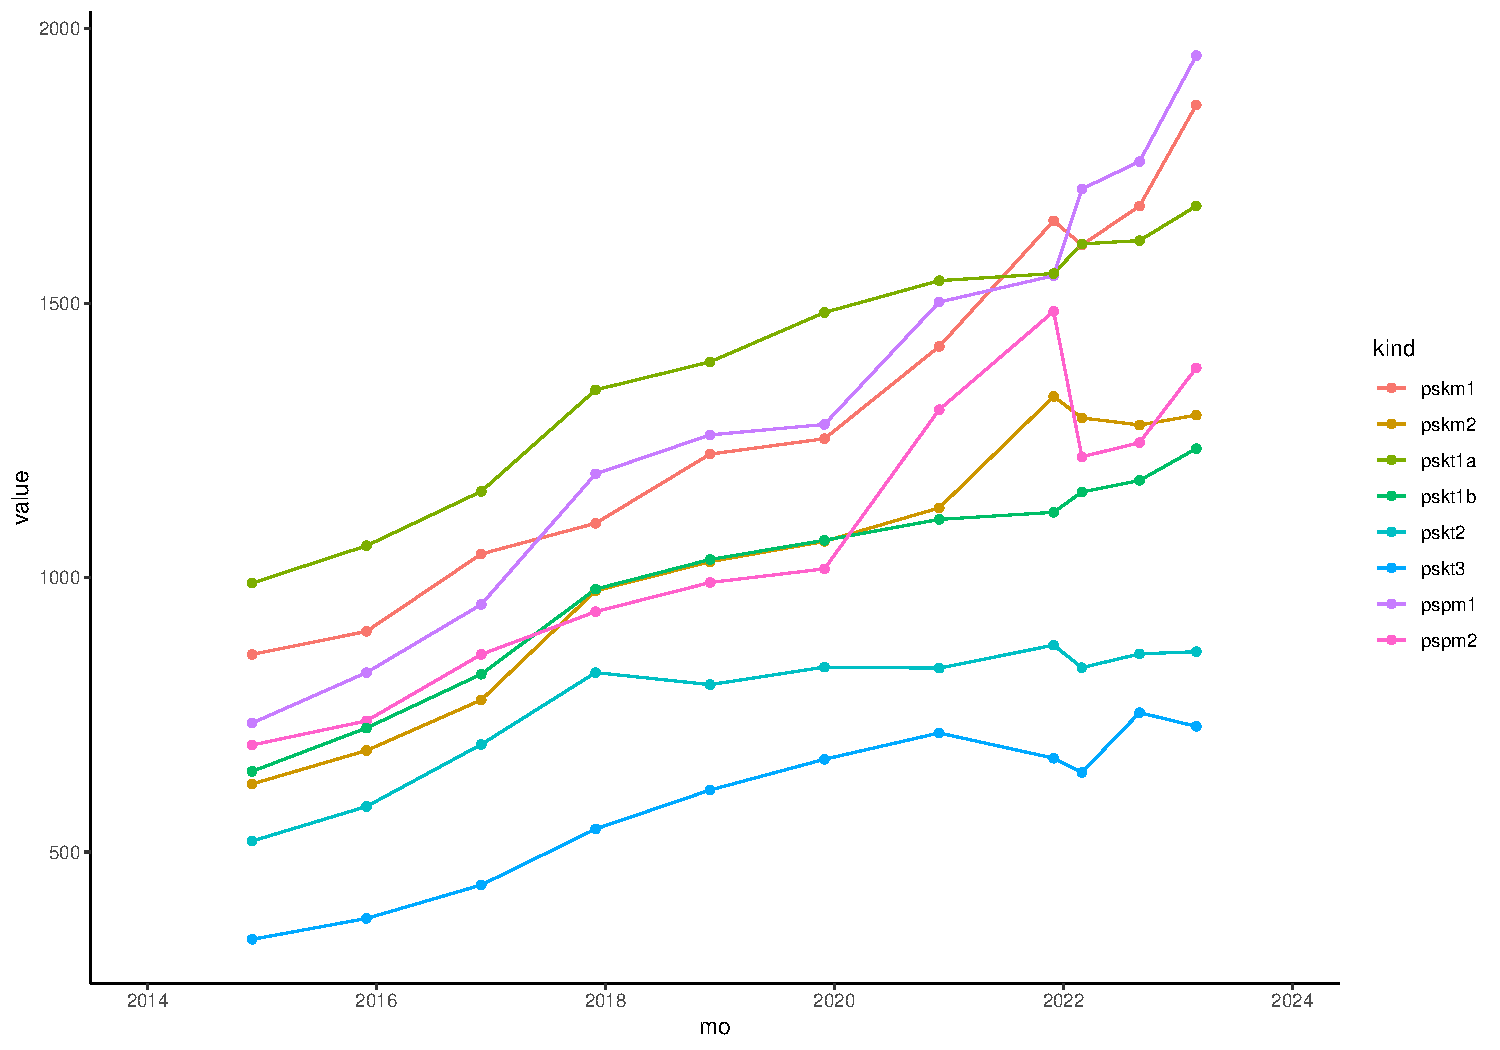
\includegraphics[keepaspectratio]{slides_files/figure-beamer/unnamed-chunk-2-1.pdf}}
\end{frame}

\begin{frame}{Base price}
\phantomsection\label{base-price}
\pandocbounded{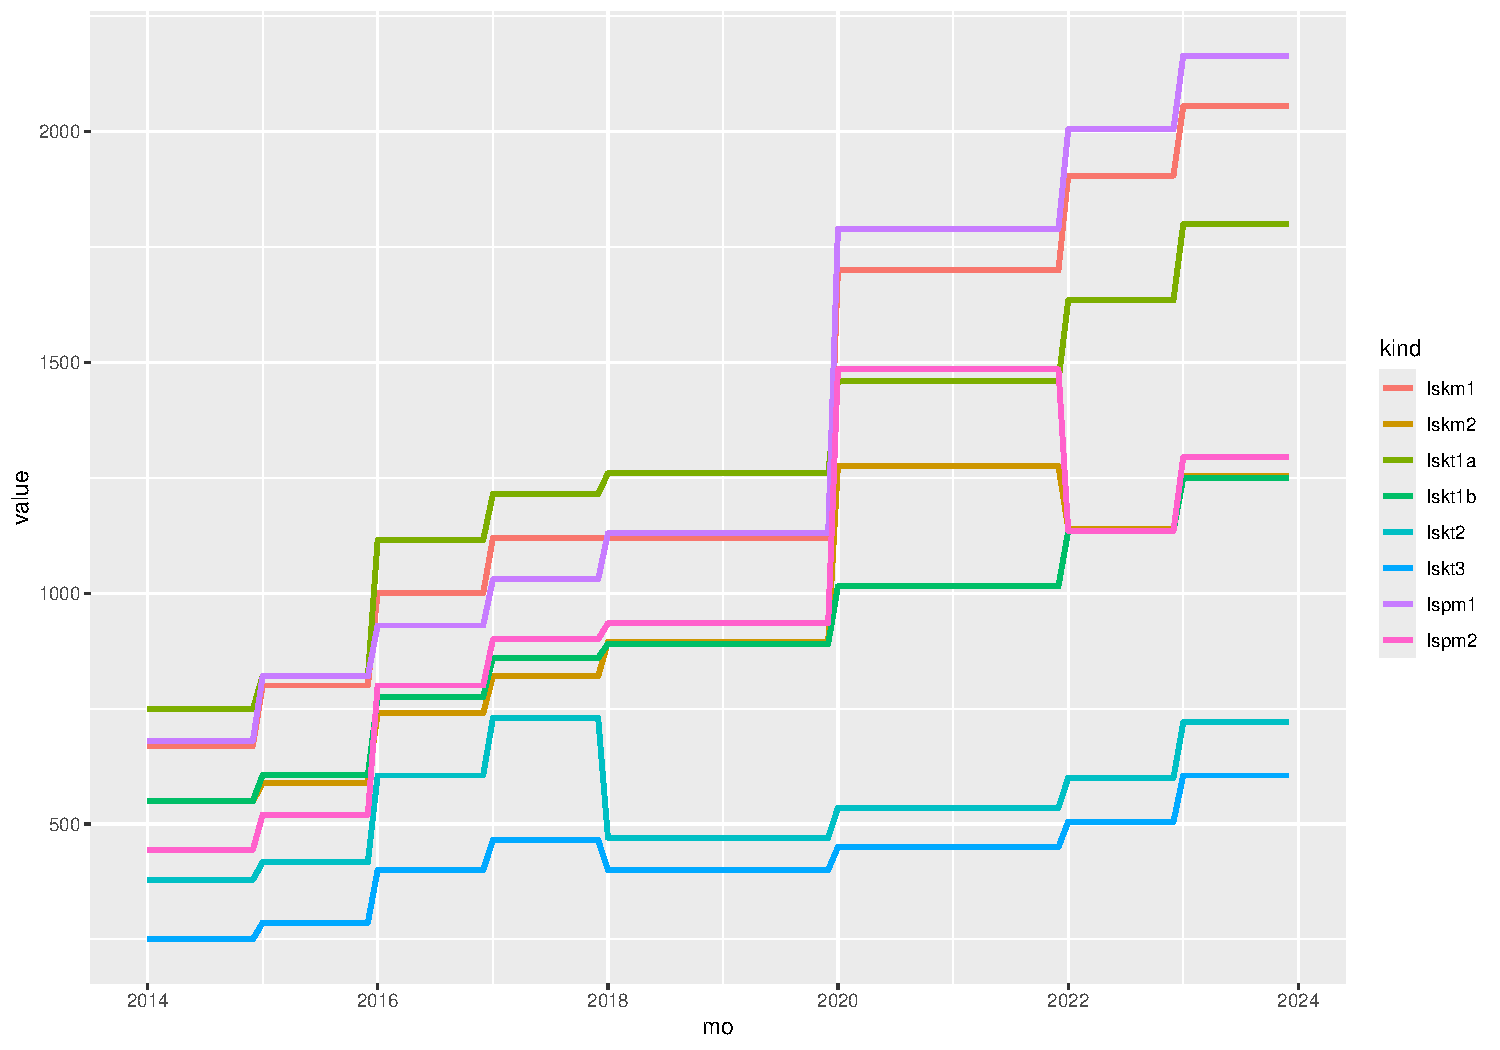
\includegraphics[keepaspectratio]{slides_files/figure-beamer/unnamed-chunk-3-1.pdf}}
\end{frame}

\begin{frame}{Demand}
\phantomsection\label{demand}
\pandocbounded{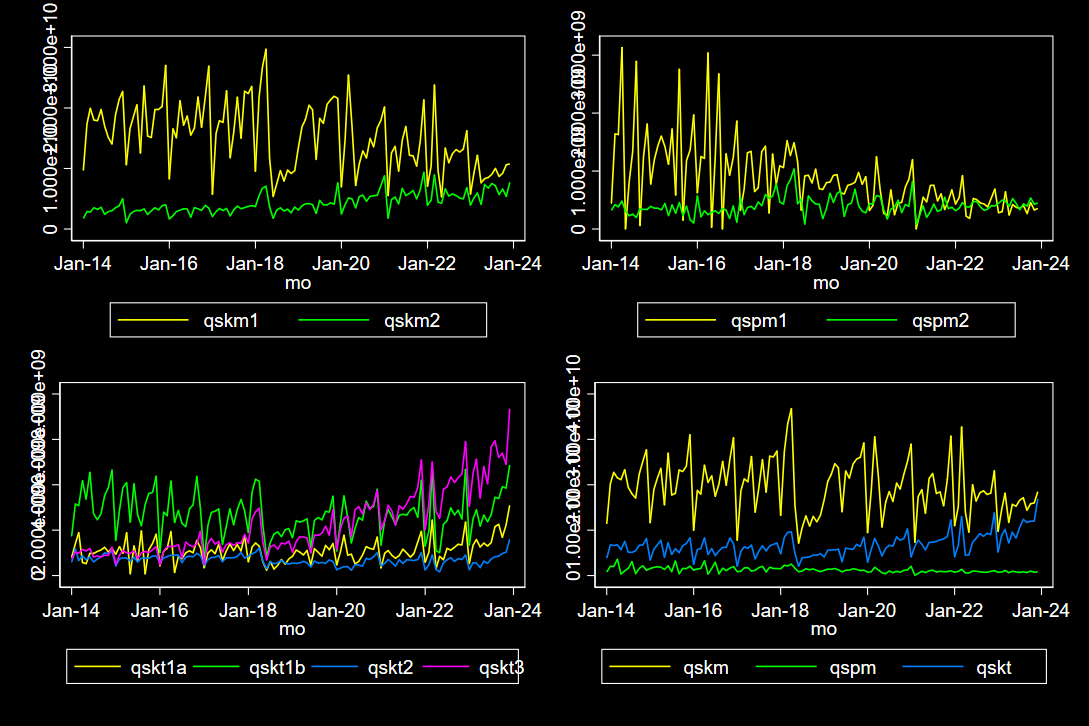
\includegraphics[keepaspectratio]{pic/demand.png}}
\end{frame}

\begin{frame}{Tariff revenue}
\phantomsection\label{tariff-revenue}
\pandocbounded{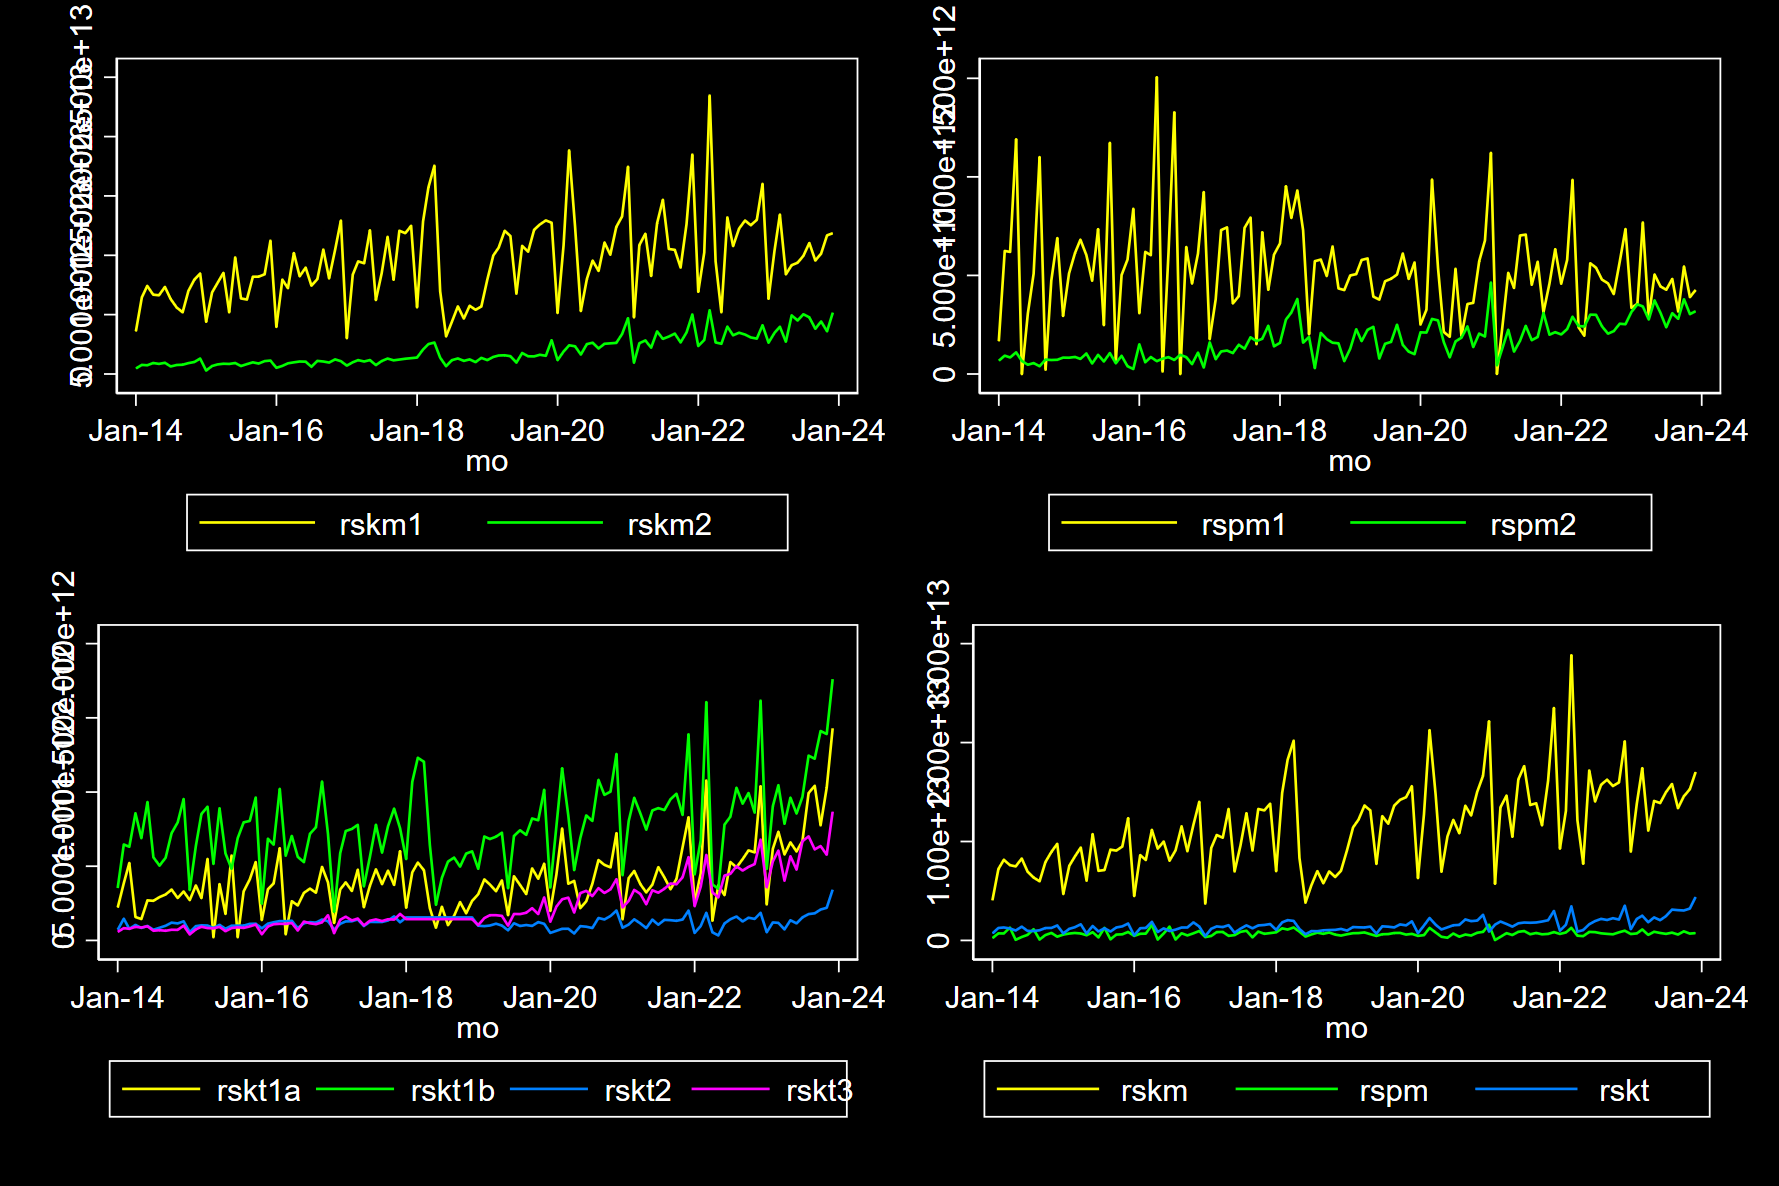
\includegraphics[keepaspectratio]{pic/revenue.png}}
\end{frame}

\begin{frame}{Market price per stick}
\phantomsection\label{market-price-per-stick}
\pandocbounded{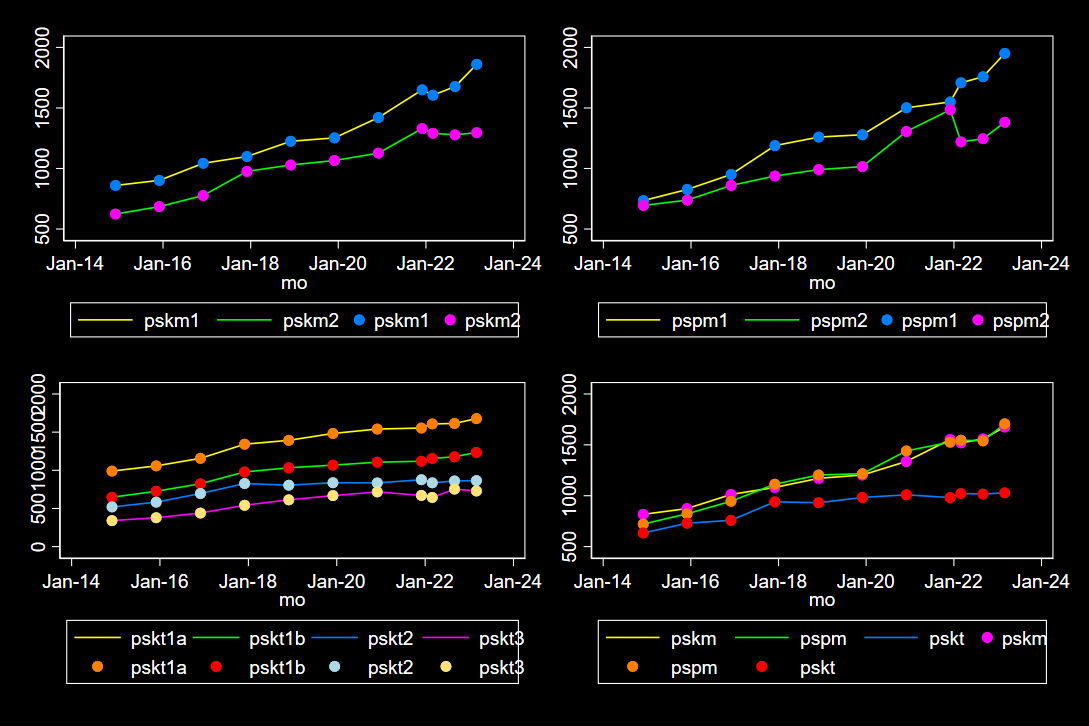
\includegraphics[keepaspectratio]{pic/htp.png}}
\end{frame}

\begin{frame}{Tariff per stick}
\phantomsection\label{tariff-per-stick}
\pandocbounded{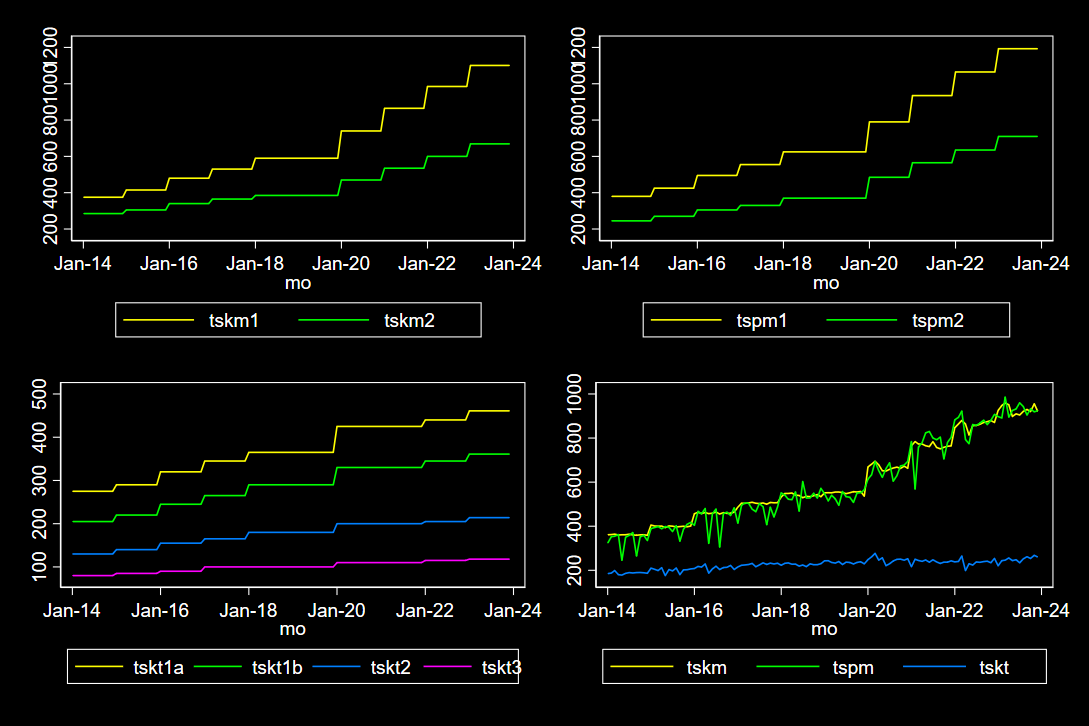
\includegraphics[keepaspectratio]{pic/tariff.png}}
\end{frame}

\begin{frame}{Analysis}
\phantomsection\label{analysis}
\begin{itemize}
\item
  There are clear negative trend on the higher tariff brackett, positive
  trend on the lower tariff brackett.
\item
  There is an important cutoff point on early 2018, coincident with the
  divergence point of the base price.
\item
  Quantity: Hand-rolled kretek (SKT) catched up with the machine kretek
  (SKM). Limited growth in revenue. Jobs is unclear, but since SKT is
  more labor intensive, it is possible we have net positive on labor
  absorption.
\item
  ``Control'' goal doesn't seem to progress.
\end{itemize}
\end{frame}

\begin{frame}{SURE reg}
\phantomsection\label{sure-reg}
\pandocbounded{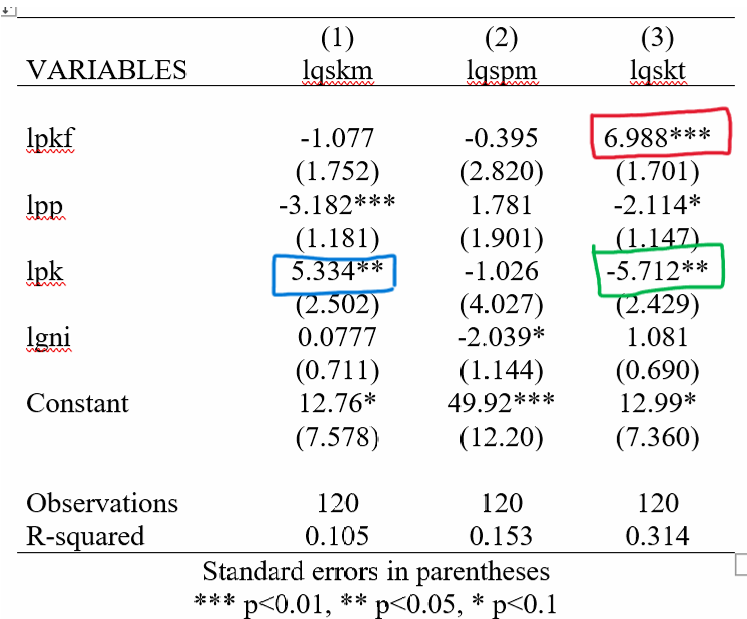
\includegraphics[keepaspectratio]{pic1.png}}
\end{frame}

\begin{frame}{Conclusion}
\phantomsection\label{conclusion}
\begin{itemize}
\tightlist
\item
  Cannot say too strongly on ``substitution'' amid price data
  limitation. E-cigs may have effects, but also no data.
\end{itemize}
\end{frame}

\begin{frame}{Referred}
\phantomsection\label{referred}
\phantomsection\label{refs}
\begin{CSLReferences}{1}{0}
\bibitem[\citeproctext]{ref-RN}
Hidayat, Budi, and Hasbullah Thabrany. 2011. {``Are Smokers Rational
Addicts? Empirical Evidence from the Indonesian Family Life Survey.''}
Journal Article. \emph{Harm Reduction Journal} 8: 6.
https://doi.org/\url{https://doi.org/10.1186/1477-7517-8-6}.

\bibitem[\citeproctext]{ref-prasetyo618}
Prasetyo, Bagus Wahyu, and Vid Adrison. 2020. {``Cigarette Prices in a
Complex Cigarette Tax System: Empirical Evidence from Indonesia.''}
\emph{Tobacco Control} 29 (6): 618--23.
\url{https://doi.org/10.1136/tobaccocontrol-2018-054872}.

\end{CSLReferences}
\end{frame}




\end{document}
